\documentclass[50pt]{article}
\RequirePackage{pdfpages}
\renewcommand{\baselinestretch}{1.4}
\RequirePackage{amsthm,amssymb,amsmath,graphicx}
\RequirePackage{color}
\RequirePackage[top=2cm, bottom=2cm, left=2.5cm, right=3cm]{geometry}
\RequirePackage[pagebackref=false,colorlinks,linkcolor=blue,citecolor=magenta]{hyperref}
\RequirePackage{xepersian}
\RequirePackage{MnSymbol}
\RequirePackage{graphicx}
\newcommand{\wid}{1.8in}
\newtheorem{theorem}{Theorem}
\newcommand{\hl}{
\begin{center}
\line(1,0){450}
\end{center}}
\newenvironment{amatrix}[1]{%
\left[\begin{array}{@{}*{#1}{c}|c@{}}
}{%
\end{array}\right]
}
\settextfont{B Nazanin}
\setlatintextfont{Times New Roman}

\begin{document}
\setLTR 




\begin{RTL}
\Large{








\begin{center}
به نام خدا

پاسخ سوالات کوییز 3
\end{center}
\hl
\textbf{سوال 1) الف) سری فوریه‌ی سیگنال 
$$x(t)=\sum_{n=-\infty}^{\infty}\delta(t-nT)$$
را به دست آورید.}

پاسخ) از تعریف سری فوریه نتیجه می شود:
\[
\begin{split}
a_k&={1\over T}\int_{T}x(t)e^{-jk{2\pi\over T}t}dt
\\&={1\over T}\int_{-{T\over 2}}^{T\over 2}x(t)e^{-jk{2\pi\over T}t}dt
\\&={1\over T}\int_{-{T\over 2}}^{T\over 2}\delta(t)e^{-jk{2\pi\over T}t}dt
\\&={1\over T}\int_{-{T\over 2}}^{T\over 2}\delta(t)e^{-jk{2\pi\over T}0}dt
\\&={1\over T}\int_{-{T\over 2}}^{T\over 2}\delta(t)dt
\\&={1\over T}
\end{split}
\]
\textbf{ب) پاسخ سیستم زیر را به ورودی فوق به دست آورید:}
\begin{center}
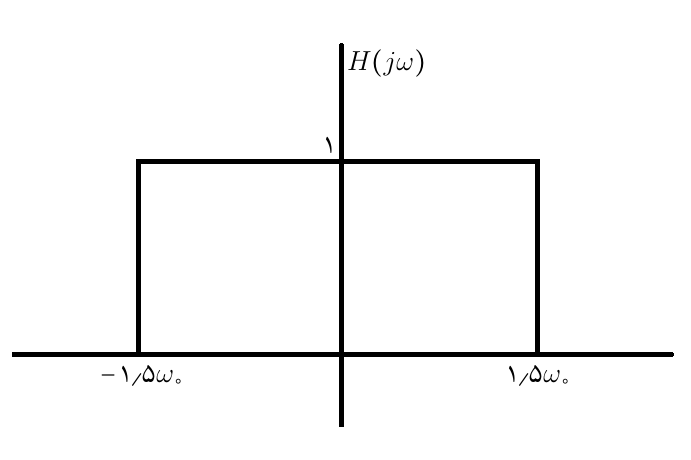
\includegraphics[width=65mm]{m6}
\end{center}
پاسخ) از آنجا که سیگنال $x(t)$ با دوره‌ی تناوب $T$ و فرکانس زاویه ای $\omega_0$ متناوب است، در اینجا تمام هارمونیک های $k\omega_0$ در طیف آن مشاهده می شوند. چون فیلتر پایین گذر مطرح شده در سوال فرکانس های زاویه ای بزرگتر از $1.5\omega_0$ را فیلتر می کند، لذا با عبور سیگنال فوق از فیلتر پایین گذر، تنها فرکانس های $0$، $\omega_0$ و 
$-\omega_0$ 
 از سیگنال عبور می کنند؛ به بیان ریاضی:
\[
\begin{split}
x(t)=\sum_{k=-\infty}^{\infty} a_ke^{jk{2\pi\over T}t}
\end{split}
\] 
\[
\begin{split}
y(t)&=\sum_{k=-\infty}^{\infty} H(jk\omega_0)a_ke^{jk{2\pi\over T}t}
\\&=a_{-1}e^{-j{2\pi\over T}t}+a_{0}e^{0j{2\pi\over T}t}+a_{1}e^{j{2\pi\over T}t}
\\&={1\over T}\left(1+2\cos {2\pi\over T}t\right)
\end{split}
\] 
در شکل زیر می توان اثر گیبس را در مورد تقریب جملات مرتبه بالای سری فوریه برای قطار ضربه مشاهده نمود:
\begin{center}
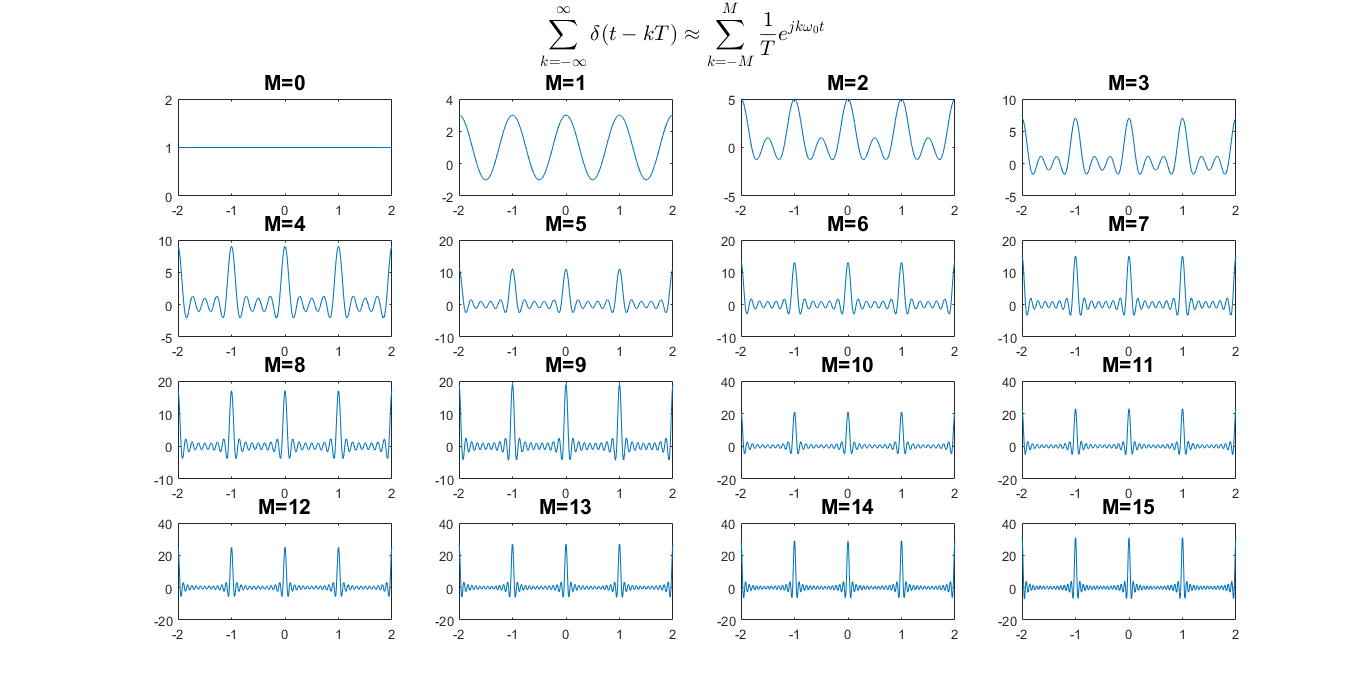
\includegraphics[width=170mm]{m9.png}
\end{center}













}





\end{RTL}



\end{document}


